
% \section{Bayesian formulation}
% From a Bayesian perspective, cognitive systems act as if they are inferring the causes of their sensations. This deduction involves anticipating sensory input based on their underlying model of the world. 

% We can formalize this by using Bayes' theorem, which is given by:
% \begin{equation}
% p(z \vert x) = \frac{p(x \vert z) p(z)}{p(x)}
% \end{equation}
% Here, \( x \) represents the observed data, and \( z \) denotes the latent variables influencing this data.

% The joint density, \( p(x, z) \), represents a generative model and is formulated as:
% \begin{equation}
% p(x, z) = p(x \vert z) p(z)
% \end{equation}
% This joint distribution combines our prior beliefs \( p(z) \) about the world and the likelihood \( p(x \vert z) \) of our observations given this world view.
% Since $z$ can be nested, we can see it as a compositional latent variable model \cite{hu_gflownet-em_2023}. 

% Given a set of observations (dataset) \( X \), the marginal likelihood or evidence is:
% \begin{equation}
% p(x) = \sum_z p_\theta(z)p_\theta (x|z)
% \end{equation}
% which is intractable and therefore often parameterized.

% The optimization challenge is to find the parameters \( \theta \) that maximize the data's log-likelihood:
% \begin{equation}
%     \mathcal{L} = \log \prod_{i=1}^{T} p(x_i) = \sum_{i=1}^{T} \log \sum_{z} p_\theta(z)p_\theta(x_i|z)
% \end{equation}








% \chapter{Technical Framework}


\section{Probabilistic Programming}

I follow the assumption that we don't start from a blank slate but from some initial concepts, here operationalized as primitives, fundamental program components. These initial primitives comprise a minimal domain-specific lanugage (DSL) and can be composed into more complex programs, which represent the causal structure generating the observations we perceive. As such, an agent learns its own DSL, which in terms of a language of thought is analogous to inferring a mental grammar and using it to learn new concepts.


\subsection{DreamCoder}
[which supercede previous models, e.g. RobustFill, DeepCoder, etc. ]
One of the most successful models in this regard is DreamCoder - a model that synthesises programs from initial primitives and a set of tasks with the objective of learning its own domain specific language \cite{ellis_dreamcoder_2021}. The model utilises a modified version of a wake-sleep algorithm introduced by Hinton to learn a generative model and a recognition network in tandem, following the paradigm of separating the world model from the inference model \cite{hinton1995wake} [reference to earlier section, sys 1,2]. The generative model learns a probability distribution over programs while the recognition network learns to map from tasks to programs in order to perform neurally guided search over the program space.
Commonly used sub-routines, are chunked and abstracted into concepts which become more accessible. This narrows the search tree immensely and enables scalability. In sum, abstraction narrows the depth, while the recognition model narrows the breadth of the search space.

Tasks can be generative (e.g. creating an image) or conditional, (input-output relation, e.g. sorting a list).
Figure \ref{fig:conc_library}(A) shows examples of tasks across different domains. 
Figure \ref{fig:conc_library}(B) shows an example, in which the task to learn is to sort a list. On the left we see the initial primitives. The shaded region shows the learned library of concepts. On the right we see the final solution, which uses \texttt{concept15} , which itself uses previously abstracted concepts. Note the difference in the length of the program using abstracted concepts vs. only initial primitives, shown beneath.

\begin{figure*}
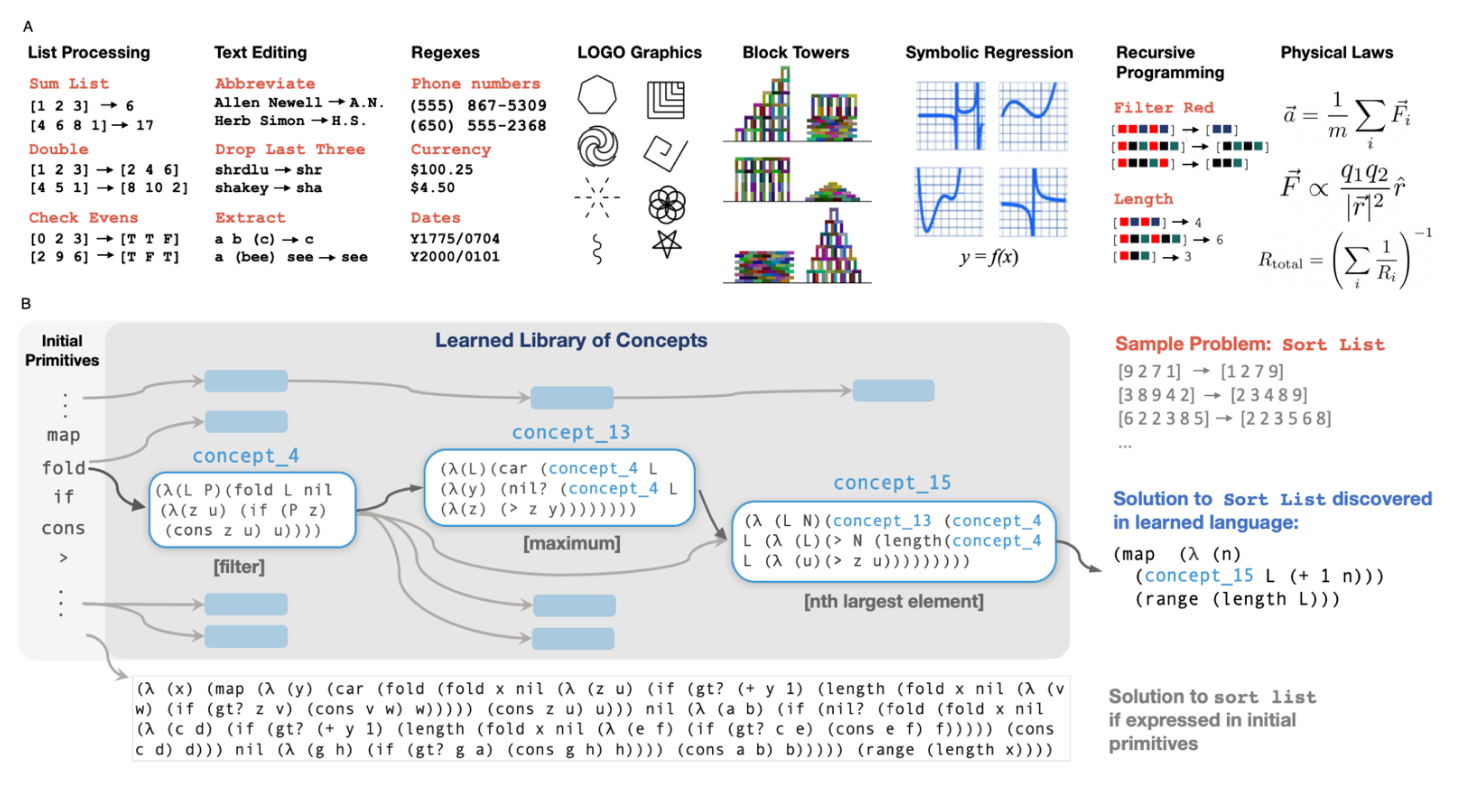
\includegraphics[width=\textwidth]{../img/conc_library.png}
\caption{(A) 8 different domains of tasks. (B) Representation of the learned library of concepts. On the left we see the initial primitives from which the concepts in the middle region are composed. On the right we see a task as input-output relations and the found solution. On the bottom is the same solution expressed only with initial primitives. Image taken with permission from the original paper \cite{ellis_dreamcoder_2021}.}
\label{fig:conc_library}
\end{figure*}



Formally, the overall objective is to find the optimal DSL \(\mathcal{D}\), which is a set of typed \(\lambda\)-calculus expressions, along with optimal weights \( \theta \) to navigate it, such as to solve a given a set of tasks \(x \in X\).

I.e. the objective is to find the joint distribution:
\[ 
    J(\mathcal{D}, \theta) = P(\mathcal{D}, \theta) \prod_{x \in X} \sum_{\rho} P(x|\rho)P(\rho|\mathcal{D},\theta) 
\]
where:
\begin{conditions*}
    P(\mathcal{D}, \theta) & Prior distribution over languages and parameters \\
    P(x|\rho) & Likelihood of task \(x \in X\) given program \(\rho\)
\end{conditions*}

Since computing \( J(\mathcal{D}, \theta) \) entails marginalizing over all programs, which is intractable, they instead marginalize over a finite beam [definition] per task \( {\mathcal{B}_x} \) which is operationalized as a lower bound on the joint density. This bound is even tighter than the ELBO [reference].
\[
    \mathcal{L}(\mathcal{D}, \theta, \{\mathcal{B}_x\}) = P(\mathcal{D}, \theta) \prod_{x \in X} \sum_{\rho \in \{\mathcal{B}_x\}} P(x|\rho)P(\rho|\mathcal{D},\theta)
\]

The model operates in three distinct phases. 

\paragraph{Wake} In the wake phase, the objective is to find the best program $\rho$ for each task $x \in X$ DreamCoder is presented with. Each task consist of one or a few ($\sim10$) examples.
The objective is to maximize \(\mathcal{L}\) w.r.t. to the beam \(\{\mathcal{B}_x\}\)

\paragraph{Sleep: Abstraction} A key component of the success of DreamCoder is the refactoring of programs. In this phase, DreamCoder consolidates new abstractions from the programs it has found during the wake phase. Experiences are replayed, and commonalities between programs are found so that they can be abstracted into new concepts to use in the future. 

% The objective is to find programs of minimum description length (MDL). 
(version space etc. )
In the abstraction phase they maximize \(\mathcal{L}\) w.r.t. \(\mathcal{D}\)
% - DreamCoder uses a new data structure based on equivalence graphs and constructed via dynamic programming which can summarize a large number of possible refactorings to the original programs.

\paragraph{Sleep: Dreaming} The objective during the dreaming phase is to train the recognition model $Q$ to perform MAP inference by both fantasies, and replays. When fantasising, programs are drawn from the learned library as a generative model. The model is then trained on the produced tasks. This ensures a large and varied data-set to learn from and encourages out-of-distribution generalisation. Replays, simply training on previously seen task-program pairs, ensures that the model improves its predictions on the actual tasks it needs to learn and doesn't forget how to solve tasks it has already solved correctly.

In dreaming they maximize \(\mathcal{L}\) w.r.t. \(\theta\).

\[
    \mathcal{L}_{\text{MAP}}^{\text{Replay}} = \mathbb{E}_{x\sim X} \left[ \log Q \left( \arg\max_{p \in \mathcal{B}_x} P(p|x, D, \theta)  \Big\lvert x \right) \right]
\]

\[
    \mathcal{L}_{\text{MAP}}^{\text{Fantasy}} = \mathbb{E}_{x \sim (D, \theta)} \left[ \log Q \left( \arg\max_{p} P(p|x, D, \theta) \Big\lvert x \right) \right]  
\]

The authors chose to optimize MAP rather than the posterior because together with their parameterization of the recognition model, this encourages to break syntactic symmetries.

The recognition model \(Q\) takes a task as input and outputs a 3-dimensional bigram transition matrix \(Q_{ijk}\), where \(i\) indexes possible children, \(j\) indexes possible parents and \(k\) indexes which argument of the parent is being generated. This parameterization was chosen as a balance between quality and efficiency.




% “We use an EM algorithm to estimate the continuous parameters of the generative model, i.e. θ. Suppressing dependencies on D, the EM updates are θ = arg max θ log P (θ) + ∑ x Eqx [log P [ρ|θ]] (3) qx(ρ) ∝ P[x|ρ]P[ρ|θ]1 [ρ ∈ Bx] (4) In the M step of EM we will update θ by instead maximizing a lower bound on log P[ρ|θ], making our approach an instance of Generalized EM.” (from building hierarchical world models , one of the DreamCoder papers)




\section{Methods}
\section{FlowCoder}




%%%%%%%%%%%%%%%%%%%%%%%%%%%%%%%%%%%%%%%%%%%%%%%%%%%%%%
%%%%%%%%%%%%%%%%%%%%%%%%%%%%%%%%%%%%%%%%%%%%%%%%%%%%%%
%%%%%%%%%%%%%%%%%%%%%%%%%%%%%%%%%%%%%%%%%%%%%%%%%%%%%%
%%%%%%%%%%%%%%%%%%%%%%%%%%%%%%%%%%%%%%%%%%%%%%%%%%%%%%
%%%%%%%%%%%%%%%%%%% DEEPSYNTH %%%%%%%%%%%%%%%%%%%%%%%%
%%%%%%%%%%%%%%%%%%%%%%%%%%%%%%%%%%%%%%%%%%%%%%%%%%%%%%
%%%%%%%%%%%%%%%%%%%%%%%%%%%%%%%%%%%%%%%%%%%%%%%%%%%%%%
%%%%%%%%%%%%%%%%%%%%%%%%%%%%%%%%%%%%%%%%%%%%%%%%%%%%%%
%%%%%%%%%%%%%%%%%%%%%%%%%%%%%%%%%%%%%%%%%%%%%%%%%%%%%%
\subsection{DeepSynth}

In their 2021 paper, Fijalkow et al. proposed a framework called "distribution-based search", in which they tackle the difficult problem of searching through a DSL to find programs matching a specification in a vast hypothesis space \cite{fijalkow_scaling_2021}.

They introduce DeepSynth \footnote{\url{https://github.com/nathanael-fijalkow/DeepSynth}}, a general-purpose program synthesizer which constructs programs from input-output examples, and a useful framework allowing us to test different models and search methods.
\paragraph{DSL} 

Here an initial DSL and suitable syntactic constraints compile into a context-free grammar (CFG), which defines the possible structures of programs within its DSL. A CFG consists of a set of production rules that describe how to generate strings (or tree structures) from a set of non-terminal and terminal symbols. It's "context-free" because the production rules are applied regardless of the surrounding symbols.

Here a CFG is used rather than the more dynamic but computationally heavy inference of variable scoping rules [explain] to determine permitted rules.
\todo[inline]{discuss that we actually need to infer the CFG but for computational reasons we just use the CFG. Otherwise, we have to find out which rules are allowed since we are dealing with types. Now is there a biologically plausible equivalent to types or is it completely a constraint of the method we are using? I suspect that there are no types. It's all dynamic. But that's okay for now.}

A probabilistic CFG (PCFG) extends a CFG by associating probabilities with the production rules. This allows the grammar to not only generate the syntactic structure of a program but also to represent beliefs about the relative plausibility or frequency of different structures. This is similar to DreamCoder's transition matrix. Here, a PCFG is used to capture prior beliefs about the distribution of programs within a domain, which guides the search and inference process towards more likely programs.

[discuss here that we are using a transformer to represent a neural PCFG?]

Programs are represented as abstract syntax trees (ASTs). An AST is a tree representation of the syntactic structure of the program, with nodes representing operations or primitives and edges representing their compositional relationships.
[insert debruin indexing definition]
[and maybe a graph]

[discuss here the difference between predicting primitives and rules?]



%%%%%%%%%%%%%%%%%%%%%%%%%%%%%%%%%%%%%%%%%%%%%
%%%%%%%%%%%%%%%%%%% DSL %%%%%%%%%%%%%%%%%%%%%
%%%%%%%%%%%%%%%%%%%%%%%%%%%%%%%%%%%%%%%%%%%%%
\paragraph{DSL}
(see appendix \ref{app:dsl})
- typed Lambda calculus 

\paragraph{Syntactic constraints}
% [show constraints]
% nb_arguments_max: maximum number of inputs
% size_max: maximum number of elements in a list
% lexicon: list of symbols that can appear (for instance range(-10,10))

\paragraph{Tasks}
We are using n? tasks, originally from DreamCoder and filtered and provided by DeepSynth.
Tasks are input-output relations in the list editing domain. [See appendix for examples]. 
we have tasks $x \in X$

% We only work with tasks of type int list -> int list. We remove examples where lists have length greater than Lmax = 10 or where one of the elements of the input or output list are not in Lin = [−30; 30].
We say that a task is solved if a program is found which satisfies all examples. The timeout of 100s only takes into account the search time and the evaluation times and not the time to query the neural network for predictions.

\begin{itemize}
    \item n dreamcoder Tasks, filtered like in DeepSynth to only have certain types.
    \item We work with list editing tasks (give a couple of examples)
    % \item from Deepsynth [We only work with tasks of type int list -> int list. We remove examples where lists have length greater than Lmax = 10 or where one of the elements of the input or output list are not in Lin = [−30; 30].
    % We say that a task is solved if a program is found which satisfies all examples. The timeout of 100s only takes into account the search time and the evaluation times and not the time to query the neural network for predictions.]
\end{itemize}


\paragraph{Rules}
I am predicting rules in the CFG, rather than primitives. I.e. edges between two symbols.




%%%%%%%%%%%%%%%%%%%%%%%%%%%%%%%%%%%%%%%%%%%%%%%%%%%%%%%%%%%
%%%%%%%%%%%%%%%%%%%%%%%%%%%%%%%%%%%%%%%%%%%%%%%%%%%%%%%%%%%
%%%%%%%%%%%%%%%%%%%%%%%%%%%%%%%%%%%%%%%%%%%%%%%%%%%%%%%%%%%
%%%%%%%%%%%%%%%%%%%%%% GFlowNet %%%%%%%%%%%%%%%%%%%%%%%%%%%
%%%%%%%%%%%%%%%%%%%%%%%%%%%%%%%%%%%%%%%%%%%%%%%%%%%%%%%%%%%
%%%%%%%%%%%%%%%%%%%%%%%%%%%%%%%%%%%%%%%%%%%%%%%%%%%%%%%%%%%
%%%%%%%%%%%%%%%%%%%%%%%%%%%%%%%%%%%%%%%%%%%%%%%%%%%%%%%%%%%
\subsection{GFlowNet}


% Incidentally, GFlowNets have been developed to construct molecules from atoms [source].

% - introduce my tasks as X, my z as rules of the CFG (discuss later why rules rather than primitives; i have to look up whether they are allowed anyways so i used the rules + order? discuss pros and cons)



Generative Flow Networks (GFlowNets), introduced by Bengio et al., are a class of generative models designed to learn to construct objects from a target distribution over complex high-dimensional spaces, particularly where explicit density estimation is challenging and diverse candidates are encouraged \cite{bengio_flow_2021}. GFlowNets learn a stochastic policy for generating sequences of actions that lead to the construction of a sample. This sampling process is done in such a way that the frequency of generating any given sample is proportional to a given reward function associated with that sample.

GFlowNets create a directed acyclic graph (DAG) over the state space, where vertices correspond to states or partial samples and edges denote transitions or adding a component to a partial sample, in which the edges carry a flow from source to targets.

In GFlowNets, the "flow" in the network corresponds to the process by which the network constructs a sample, which can be thought of as a path in a graph where nodes are partial samples, and edges correspond to adding a component to the partial sample. The network is trained such that the flow into any completed sample is proportional to its reward.

[put a diagram here? of partially constructed ASTs]

The core training objective for a GFlowNet is to satisfy the flow matching constraint. The idea is to ensure that the flow into any state (a partially constructed sample) should match the flow out of it, given the reward associated with complete samples. The flow here refers to the expected transitions into or out of a state under the model's stochastic policy. 

Formally, a state \( s \) represents a partial object a certain stage in the generative process. A trajectory \( \tau \) is a sequence of states \( s_0, s_1, ..., s_T \) that the model traverses from an initial state \( s_0 \) to a terminal state \( s_T \), where the target structure is complete.

A trajectory \( \tau \) is formed by a sequence of actions \( a_1, a_2, ..., a_T \), where each action \( a_t \) transitions the model from state \( s_{t-1} \) to state \( s_t \). The sequence of actions is governed by a policy \( \pi \), which defines the probability of choosing a particular action given the current state.

% A reward is used to evaluate complete objects [could also be partial]. 

The flow \( F(\tau) \) of a trajectory \( \tau \) is defined as the product of the probabilities of each transition along the trajectory, multiplied by the reward \( R(s_T) \) of the terminal state, normalized by a partition function \( Z \).

\begin{equation} \label{eq:flow}
    F(\tau) = \frac{R(s_T)}{Z} \prod_{t=0}^{T-1} \pi_\theta(s_{t+1} | s_{t})
\end{equation}

The partition function \( Z \) ensures that the sum of flows over all possible trajectories equals one, effectively normalizing the distribution. Since we don't know \( Z \), we can estimate it by parameterizing it as \( Z_{\theta} \).

The flow matching constraint enforces that for any given non-terminal state \( s \), the total flow into \( s \) must equal the total flow out of \( s \):

\begin{equation} \label{eq:flow_match}
    F(\tau) = F(\tau')
\end{equation}

where \( F(\tau') \) is the reverse trajectory.

We can utilize this property to create a suitable loss function to train the GFlowNet. Combining equations \ref{eq:flow} and \ref{eq:flow_match} gives us:

\begin{equation}
    \frac{R(s_T)}{Z_\theta} \prod_{t=0}^{T-1} \pi_\theta(s_{t+1} | s_{t}) = \frac{R(s_0)}{Z_\theta} \prod_{t=0}^{T-1} \beta_\theta(s_{t} | s_{t+1})
\end{equation}

Here \( \beta \) is the backward policy, predicting parent states. 
The initial state \(s_0\) has the total flow and no reward, we can rewrite it and get:

\begin{equation}
    Z_{\theta} \prod_{t=0}^{T-1} \pi_\theta(s_{t+1} | s_{t}) = R(s_T) \prod_{t=0}^{T-1} \beta_\theta(s_{t} | s_{t+1})
\end{equation}

We can now take the log on both sides:

\begin{equation}
    \log \left(Z_{\theta} \prod_{t=0}^{T-1} \pi_\theta(s_{t+1} | s_{t})\right) = \log \left(R(s_T) \prod_{t=0}^{T-1} \beta_\theta(s_{t} | s_{t+1})\right)
\end{equation}


This can be rearranged to:

\begin{equation}
    \log Z_\theta + \sum_{t=0}^{T-1} \log \pi_\theta(s_{t+1}|s_{t}) = \log R(s_T) + \sum_{t=0}^{T-1} \log \beta_\theta(s_{t}|s_{t+1})
\end{equation}

The trajectory balance loss is the squared difference:

\begin{equation}
    \mathcal{L}_{TB} = \left(\log Z_\theta + \sum_{i=0}^{T-1} \log \pi_\theta(s_{t+1}|s_{t}) - \log R(s_T) - \sum_{t=0}^{T-1} \log \beta_\theta(s_{t}|s_{t+1})\right)^2
\end{equation}


In order to mitigate the computational [cost], I am embedding all rules rather than primitives, such that each rule is unique. Thus, every predicted node (rule) has exactly one parent, in other words, I am essentially linearizing the tree. Therefore, $\beta$ will always be $1$ and can be disregarded from the equation. 
Moreover, since we are solving tasks \( x \in X \), we have a conditional reward distribution $R(s_T|x)$, as well as a conditional forward policy $\pi_\theta(s_T|x)$ and partition function $Z_\theta(x)$.
This gives us the final loss:

\begin{align}
     \mathcal{L}_{TB} = \left(\log Z_\theta(x) + \sum_{t=0}^{T} \log \pi_\theta(s_{t+1}|s_{t}, x) - \log R(s_T \vert x)\right)^2
\end{align}     




\subsection{Expectation-Maximization}
% https://github.com/GFNOrg/GFlowNet-EM/

% I am following the idea of separating the world model from the inference model (system 1 and 2) and use an expectation maximization algorithm [GFN-EM, DC, ... ] to train the models.

The core principle of Expectation-Maximization (EM) involves an iterative two-step process: the Expectation (E) step computes an expectation of the log-likelihood evaluated using the current estimate for the parameters, and the Maximization (M) step, computes parameters maximizing the expected log-likelihood found on the E step.

In the E-step I optimize the recognition model, i.e. the forward policy of the GFlowNet that is proportional to the posterior and to the reward function. 

Here, I'm sampling real data as well as a trajectory and use the trajectory balance loss to update the parameters of the forward policy.

In the M-step I sample a trajectory and only use the reward to update the parameters of the generative model.


INCLUDE PSEUDOCODE



Solving the joint optimization problem is difficult. I'm taking inspiration from DC and GFN-EM to use wake-sleep to train the models.
\paragraph{Replay}
In replay, I train the recognition model to not forget previously solved tasks.
\paragraph{Fantasy}
[also generative model?]
In fantasy I train the recognition model to solve out of distribution tasks, so it learns to extrapolate to unseen data.













































%%%%%%%%%%%%%%%%%%%%%%%%%%%%%%%%%%%%%%%%%%%%%%%%%%%%%%%%
%%%%%%%%%%%%%%%%%%%%%%%%%%%%%%%%%%%%%%%%%%%%%%%%%%%%%%%%
%%%%%%%%%%%%%%%%%%%%%%%%%%%%%%%%%%%%%%%%%%%%%%%%%%%%%%%%
%%%%%%%%%%%%%%%%%%%%%%%%%%%%%%%%%%%%%%%%%%%%%%%%%%%%%%%%
%%%%%%%%%%%%%%%%%%%%%% MODEL %%%%%%%%%%%%%%%%%%%%%%%%%%%
%%%%%%%%%%%%%%%%%%%%%%%%%%%%%%%%%%%%%%%%%%%%%%%%%%%%%%%%
%%%%%%%%%%%%%%%%%%%%%%%%%%%%%%%%%%%%%%%%%%%%%%%%%%%%%%%%
%%%%%%%%%%%%%%%%%%%%%%%%%%%%%%%%%%%%%%%%%%%%%%%%%%%%%%%%
%%%%%%%%%%%%%%%%%%%%%%%%%%%%%%%%%%%%%%%%%%%%%%%%%%%%%%%%
\section{Model}


\paragraph{generative model}
As we have seen in the Transformer part, self-attention is an algorithm which lets the transformer learn syntactic and semantic structure from its data. This inductive bias is stronger than the purely syntactical nature of the PCFG.
[neural PCFG, etc. ]

The GEN model is. a transformer


\paragraph{Recognition model}
while the recognition model si a MLP on top of the transformer. The partition function Z is also parameterized sa a MLP ib top of the transformer. 
% the recognition model is a mlp. the exact parameterearzation can be found in app:par 
% same for Z
% $q(z|x_i)$ is parameterized as a neural network. The goal is to approximate $q$ such that $q(z|x_i) \propto p(z|x_i)$, i.e. the true posterior. 


\paragraph{IOEncoder}
Task embedding 
The IOEncoder is tasked with encoding input-output (IO) pairs into continuous vector representations.
It encodes an IO pair into a flat sequence with special tokens ('IN' and 'OUT') indicating the boundary between input and output.
- Show the exact model (transformer, how many layers, etc. and make a table of that? or is it already in the table? )

- explain how tasks are created (and that it also takes time if we create new tasks from scratch for replay and fantasy.)

from Deepsynth[Input encoding Each list in the examples is encoded in a naive way by mapping each element of Lin to [0, 60]. We additionally use two special symbols PAD and NOPAD, leading to a fixed size encoding of a list into a vector of size 2Lmax. Hence an example is encoded as a tensor of shape (ninputs,2Lmax) where ninputs is the number of inputs in the example.]

- I deviate from the DeepSynth and DreamCoder implementation to make it more suitable for a Transformer.
Therefore, I \dots


See \ref{table:params} for parameter details (i think there are more, check it.). 



\subsection{RuleEncoder}
State embedding
- DSL and syntactic constraints are compiled into a CFG
The RuleEncoder is designed to transform programming rules derived from a Context-Free Grammar (CFG) into continuous vector representations, or embeddings.
in order to have semantics and not just syntax, i.e. use additional information of the CFG, I create a neural PCFG. (see kim)
In each step, I predict the next rule from the cfg, until a trajectory is done. This means that a state is a trajectory of rules and a program is represented as such a list.
Other ideas to represent ASTs are GNNs, or Tree-Transformers [which were explored, but the computational complexity gets higher [source]. also distributed representations of aggregations are an option like in GFN-EM.], however, I settled on using a regular transformer, since it has been shown that it can learn tree structures implicitly, through positional encoding and also [source] show that the performance is similar.
since we are representing trees, it might be beneficial to embed programs in hyperbolic space [see conceptual spaces]. 
There are other ways to embed the cfg, [e.g. see kim].


since im using the cfg to extract only the allowed rules, it was easier to embed rules rather than primitives, 

Rules could be encoded including additional information like tree depth, arg idx, parents, siblings, etc. 
since an AST is two dimensional, there are many expansion orders. 
my model is a transformer with a MLP on top to predict logits for the rule. I could have another, to predict the position to attach the next node. Other than that if i only embed primitives instead of rules, 
We could use a GNN and do both node and edge prediction. 
Otherwise, we also need to decide expansion order since rules are context free, i.e. if we only predict the rule there may be multiple parts of the tree where this could be applied to. However, there may be benefits in expanding in different orders. We could apply a second GFN to predict the next best node to expand.
In the cfg we have terminals and nonterminals

When constructing an AST, it can be expanded in various orders.
E.g. we could predict the tree bottom up, i.e. predict terminal nodes and then connect them progressively. The benefit of this is that we can evaluate partial expression. However, once a partial tree is predicted, the other arguments of the function are dependent on it so we have to keep expanding nodes upwards until ...

since we are representing the tree as an array of rules, so that we can use them with transformer, we need to reformat it back into a tree to evaluate it. i.e. we need to fisrt construct it and then go through it again for evaluation. this slows down the computation. 


- heapsearch, evaluation, using sub-trees, etc. 
Another expansion is using a depth first search (DFS) [source] approach (note that this is not about searching through the CFG, but constructing the AST). Since we are essentially linearising a tree when giving it as input to the transformer, the transformer has additional order information, which in combination with positional encoding lets it learn better. 

Moreover, in the original GFN, as explained above [ref] we need a prediction for the backward logits. however, since we are creating trees top-down, every state has exactly one parent. therefore, we can make the calculations simpler and omit the backward logits. 
In general, it might not be a bad idea to include it since we can use it to do other kinds of inferences [e.g. in using subtrajectory balance].















\begin{enumerate}
    \item We get a task (how do we sample?)
    \item the task gets encoded
    \item goes through transformer, 
    \item GFN predicts a rule, which is now the next state
    \item we repeat this until we have a program
    \item construct the program from the array of rules
    \item evaluate program against ideal output
    \item calculate TB loss
    \item Update model
\end{enumerate}
\begin{enumerate}
    \item same as above, but different loss. update generative model rather than 
\end{enumerate}

\begin{itemize}
    \item Data augmentation
    \item Self-supervised learning
    \item Sleep phase
    \item Replay 
    \item Fantasy
    \item Overfitting
    \item Loss optimality. Quality vs Quantity
    \item Explain CFG, parameters like program depth, sizemax etc. 
    \item How many programs can actually be created?
    \item Exploration
    \item What is the generative model? The CFG or the Transformer?
    \item Minimum description length (how is that achieved in DC (MAP?) and DS(Expectation of number of programs created before a solution is found)?)
    \item syntactic symmetries, symmetry breaking, show DC MAP vs POST, avoid adding 0, mult 1, etc. 
    \item In the paper they say they produce programs up to depth 6
    \item We want to find a probability distribution that is proportional to a reward.
    \item Explain the parameterization. I.e. we could parameterize the rules vs the primitives. 
    \item Write about the marginalization. Can we marginalize the CFG? How does DC do it? (they only marginalize over a beam) 
    \item Do we want multiple solutions? MAP vs MLE + how could we convert one to another (Talk also about DC, and why they chose MAP)
    \item Surfaces and Essences analogy example abc:xyz :: abd: (wyz/ xya) 
    \item Neural PCFG (Compare to Neural PCFG from Rush and GFN-EM)
    \item what is the difference between amortized EM and GFlowNet EM?
    \item I think GFlowNet-EM is using a neural PCFG as a generative model. 
    \item write about tractability
    \item should there be one or multiple world models?  what is the world model here? the PCFG? i.e. the generative model? 
    \item Write about context free grammars. number of possible derivations.
    \item learning your own dsl
    \item should there be one dsl or multiple?
    \item it could be e.g. having multiple representations/ models of the world and then a model on top of that which tells you which model is useful. This reminds me of society of mind and also of neural darwinism. World models may be competing with one another. 
    \item Sticking with a task for how long, before switching
    \item Evaluation of variables
    \item Now we are predicting rules, and encoding them individually. We could also use their features like depth, arg idx etc. to encode them 
    \item Why we dont need backward logits
    \item when we only predict rules, it may be ambiguous. The same rule could expand different parts of the tree. That's why DFS
    \item we want to show that using the transformer for semantics makes sense, therefore we need to show that it learnt program embedding. relating tasks to programs and also relationships between tasks and relationships between programs. Also relate that to the embeddings of tasks in DC, which shows that similar tasks are approximately in the same space.
    \item Explain what exactly this task shows or is supposed to represent. Algorithmic thinking, or any type? Dehaene, (also sensory data pattern prediction machine paper)
    \item explain what the batches do
    \item I embed all the rules (check this with neuralPCFG and maybe embed the cfg so that you have a better generative model) (not the depth, arg number etc. )
    \item I am searching for the posterior (aligning with active inference), because i want diverse solutions, i.e. i want to learn the solution space for each task, multiple modes, not just the max mode. (how does this compare to MDL)
    \item does the model align with FEP
    \item If the CFG is generative, is that not a causal model? can there be a generative causal model? be clear about those terms. 
    \item What do we need? Differently from the other models which do not embed programs (they do have a programencoder, so what is that then? the output). The output tensor is encoded as a program. The programs themselves are never embedded. What is the difference?
    \item Reasons for using a GFlowNet 
    \item Transformer allows for semantic relationships (although we still don't use control or data flow, but we could in principle)
    \item We want to approximate a multimodal distribution, unlike DreamCoder in which the MAP estimate refrains from finding semantically equal but syntactically different solutions.
    \item Implicit vs explicit generative model, neuralPCFG, embedding rules. 
    \item MAP vs  (convergent vs divergent thinking.)
    \item One shot (predicting bigram transition matrix) vs trajectory (predicting logits in each step)
    \item argument for attention and why it might be necessary to capture semantics.
    \item transformers learn nested relationships (see chapter wolfram) (relationships of increasing complexity)
\end{itemize}
    



% In DreamCoder, they do something similar. They have a generative model in the form of a PCFG, and a recognition model which takes a task as input and outputs a bigram transition tensor, which serves as a policy over actions. Here $Q$ is a conditional distribution, a mapping between IOs and programs. This is essentially an encoding of programs as tasks, which can also be seen in their visualization of task embeddings.
% The PCFG is completely syntactical.
% So they train the model to predict better weights and then search in the pcfg enumeratively. 

% for each task they have a beam, which they marginalize over. Is that not the same essentially as a GFN????

% - What is the prior, likelihood, etc. how is it operationalised

% An EM algorithm is used to estimate the parameters of the generative model.


\begin{itemize}
    \item Nathaniel compare enumeration based methods with sampling methods. quality vs quantity.
    \item If the sampler is good enough, there is no need for search
    \item does anything prevent DC from training further, improving the recognition model, making it a sampler? (it doesn't take partial programs, it only takes tasks.)
    \item We have seen that if a GFN is trained well enough, it should act as a really good sampler. So we use that 
\end{itemize}


Code available at \url{https://github.com/R1704/master_thesis}
% In this work, I am implementing a novel program synthesizer, which integrates with the DeepSynth framework. 

% I am separating the generative model (world model) from the inference model. And am using a full transformer.
% Tasks are encoded using the transformer encoder. [explain in detail], which states are encoded using the decoder. A state is represented as a rule of the cfg.
% at each step of the trajectory, the combined inputs are used for the forward logit network to predict logits over possible actions which are then added to the state.










% Make a diagram of the pipeline, sample forward, until a state is constructed, evaluation, etc. maybe also with sleep

























































































































































\begin{algorithm}
\caption{Function get\_next\_rules}
\begin{algorithmic}[1]
\Function{get\_next\_rules}{$self, S, depth$}
    \State \Return $\left\{ (S, p) \mid p \in \text{self.cfgs[depth].rules}[S].\text{keys()} \right\}$
\EndFunction
\end{algorithmic}
\end{algorithm}

\begin{algorithm}
\caption{Function get\_mask}
\begin{algorithmic}[1]
\Function{get\_mask}{$self, rules$}
    \State $mask \gets [1 \text{ if } rule \text{ in } rules \text{ else } 0 \text{ for } rule \text{ in } self.model.state\_encoder.rules]$
    \State $mask \gets \text{torch.tensor}(mask, \text{device=device})$
    \State \Return $mask$
\EndFunction
\end{algorithmic}
\end{algorithm}

\begin{algorithm}
\caption{Function sample\_program\_dfs}
\begin{algorithmic}[1]
\Function{sample\_program\_dfs}{$self, batch\_IOs, depth, \epsilon=0., \beta=1.$}
    \State Initialize states, total\_forwards, final\_logZs, frontiers, programs
    \While{\textbf{any}(frontiers)}
        \State Calculate forward\_logits, logZs
        \State Handle exploration and tempering
        \For{$i \gets 0$ \textbf{to} $\textbf{len}(batch\_IOs)-1$}
            \If{frontiers[i]}
                \State Handle rule sampling and state update
            \EndIf
        \EndFor
    \EndWhile
    \If{\textbf{not any}(frontiers)}
        \State Reconstruct final programs
        \State \Return final\_logZs, total\_forwards, reconstructed, states
    \EndIf
\EndFunction
\end{algorithmic}
\end{algorithm}




\subsubsection{Reward}

In order to train the model, we need an informative reward, i.e. it should provide a gradient.
Of course we cannot just use the actual program to compare it with. In deepsynth they train by using the cross entropy loss between the nueral network aoutput and an encoding of the solution program. In reality we do not have the correct solution [think about this. we do also learn from others. so its not entirely out of question.]. Instead, we can only compare the real and predicted output. However, there are a few methods we can try to turn the comparison of sequences into a reward. Since we are working with numeric list editing, ...
After some initial experiments of using a Hamming distance, comparing embeddings using cosine similarity, mutual gain, I decided to use an edit distance, more specifically, Levenstein edit distance (which is continuous rather than discrete.) 

Another idea is to use an energy based model, which essentially is a model that learns to predict the reward. however, this increases the computational overload and was not necessary for this toy problem.

The edit distance, often referred to as the Levenshtein distance, is a measure of the similarity between two strings. Specifically, it quantifies the minimum number of single-character edits (i.e., insertions, deletions, or substitutions) required to transform one string into another.
Given two strings \( s \) and \( t \) of lengths \( m \) and \( n \) respectively, the Levenshtein distance \( d(s, t) \) is defined as the cost of the cheapest sequence of edits needed to transform \( s \) into \( t \). 
The Levenshtein distance can be efficiently computed using dynamic programming. The idea is to construct a matrix where each cell \( (i, j) \) represents the cost of transforming the first \( i \) characters of \( s \) into the first \( j \) characters of \( t \). 

The formula for filling in the matrix is:
\begin{enumerate}
    \item If \( i = 0 \), then \( d(i, j) = j \) (cost of adding \( j \) characters).
    \item If \( j = 0 \), then \( d(i, j) = i \) (cost of deleting \( i \) characters).
    \item Otherwise:   \[
        d(i, j) = \min \begin{cases} 
        d(i-1, j) + 1 \\ 
        d(i, j-1) + 1 \\ 
        d(i-1, j-1) + \text{cost}(s_i, t_j) 
        \end{cases}
        \]
        where \( \text{cost}(s_i, t_j) \) is 0 if \( s_i = t_j \) and 1 otherwise.
\end{enumerate}

The value of \( d(m, n) \) will then be the Levenshtein distance between \( s \) and \( t \).


Since the Levenshtein distance returns a discrete value, I normalize it over the max length of the sequences, and since there may be more than one example per task, I average it over all examples.
Quantifying the result in this way gives us quite a good estimate of the model's capabilities. E.g. when we have two lists [1,2,3] [1,2,3] ...
















































%%%%%%%%%%%%%%%%%%%%%%%%%%%%%%%%%%%%%%%%%%%%%%%%%%%%%%%%%%%%
%%%%%%%%%%%%%%%%%%%%%%%%%%%%%%%%%%%%%%%%%%%%%%%%%%%%%%%%%%%%
%%%%%%%%%%%%%%%%%%%%%%%%%%%%%%%%%%%%%%%%%%%%%%%%%%%%%%%%%%%%
%%%%%%%%%%%%%%%%%%%%%%%% Design %%%%%%%%%%%%%%%%%%%%%%%%%%%%
%%%%%%%%%%%%%%%%%%%%%%%%%%%%%%%%%%%%%%%%%%%%%%%%%%%%%%%%%%%%
%%%%%%%%%%%%%%%%%%%%%%%%%%%%%%%%%%%%%%%%%%%%%%%%%%%%%%%%%%%%
%%%%%%%%%%%%%%%%%%%%%%%%%%%%%%%%%%%%%%%%%%%%%%%%%%%%%%%%%%%%

%%% Training
\begin{itemize}
    \item The model was trained on the filtered DC tasks 
    \item with a random 50 50 train test split
    \item batch size 4
    \item syntactical constraints
    \item GPU NVIDIA Tesla A100
    \item 2000 e-m steps 
    \item with thresholding
    \item 
\end{itemize} 

%%% Inference
\begin{itemize}
    \item In inference, the model still has batchsize 4
    \item syntactic constraints
    \item we give it a 100 inference steps (400 programs are created)
    \item run on all 145 tasks
    \item 
\end{itemize}











% I am training the model on about a quarter of the tasks, 37 of 145 [see appendix].
% im training on batches of size 4 with the same task the whole batch. This is for efficiency. This means that in training, I am solving the tasks n_epochs x e_steps x m_steps x batch_size times. Here 5 x 2000 x 2000 x 4 = 80.000.000 times per task. (compare to DC 400.000.000 programs per task)
% we can solve 28/31 ? of all tasks:

% I keep training on the second half of the train data and again doing inference on all.
% Check again.






















%%%%%%%%%%%%%%%%%%%%%%%%%%%%%%%%%%%%%%%%%%%%%%%%%%%%%%%%%%%%
%%%%%%%%%%%%%%%%%%%%%%%%%%%%%%%%%%%%%%%%%%%%%%%%%%%%%%%%%%%%
%%%%%%%%%%%%%%%%%%%%%%%%% Results %%%%%%%%%%%%%%%%%%%%%%%%%%
%%%%%%%%%%%%%%%%%%%%%%%%%%%%%%%%%%%%%%%%%%%%%%%%%%%%%%%%%%%%
%%%%%%%%%%%%%%%%%%%%%%%%%%%%%%%%%%%%%%%%%%%%%%%%%%%%%%%%%%%%
%%%%%%%%%%%%%%%%%%%%%%%%%%%%%%%%%%%%%%%%%%%%%%%%%%%%%%%%%%%%
\subsection{Results}

\subsubsection{Training}
\begin{itemize}
    \item How many programs are solved?
    \item Diverse solutions?
    \item did the model converge? 
    \item how long did it take to find a program?
    \item what are the other programs created?
\end{itemize}





inference:
- (especially when the model solved extrapolated tasks, were these programs found before in training?)
- how long to solve tasks? 
- if solved, how often?
- which other programs were created when trying to solve a task?

\begin{itemize}
    \item Speed/ how long did it take to solve the tasks
    \item How long does it take to solve a program?
    \item Which tasks are solved
    \item Which tasks are not solved, why?
    \item Comparison with deepsynth
    \item How many programs are uniquely created? vs solved.
	\item Make a histogram of all the programs. Can we make it over time? I.e. for each program we should see how often it is created over time. 
    \item The program is not loss optimal, i.e. we may get stuck in a local minimum
    \item Compare to baseline (Uniform PCFG?)
    \item my hopes would be that similar programs are embedded close in space. - how can we check that?
    \item visualize task embeddings (from DC) and the according programs. Maybe take the programs with the highest reward even if it didn't solve it
    \item Visualize rule embeddings. what would i expect? 
    \item Training vs. inference (check the speed of finding solution before and after training and compare. Is the inference really fast? then it means that in principle we can get a good approximation to the reward)
    \item In Deepsynth they train on 10.000 examples from a random PCFG. then the model is shown the examples once, and they search through the PCFG for n seconds until they hopefully find the correct program. the problem is that the randomly created programs suck. they don't resemble real world programs in the slightest. if i train the network directly on the tasks, then yeah, were training it first which should be amortized and then inference should be fast.
    \item Check the DC paper. What can we actually compare?
\end{itemize}




We can see that even after several training rounds, the model still explores alternative solutions. This indicates. The human analogue is divergent thinking. 


\subsubsection{Inference}






\subsubsection{Embeddings}
We can visualize embeddings using  t-SNE (t-distributed Stochastic Neighbor Embedding). The goal of t-SNE is to group similar points together and separate dissimilar ones. If certain tasks are clustered together on the plot, this suggests that the model finds them to be similar in some way.






\begin{figure}[H]
    \centering
    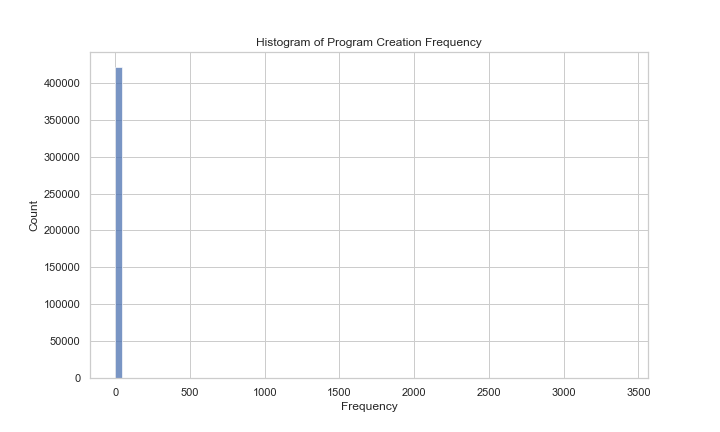
\includegraphics[width=\textwidth]{../img/plot_program_creation_frequency.png}
    \caption{}
    \label{fig:program_creation_frequency}
\end{figure}
Figure \ref{fig:program_creation_frequency} presents a histogram illustrating the frequency distribution of program creations across various tasks. This visualization aids in understanding the commonality of specific programs in solving different tasks, highlighting the most frequently utilized programs. The x-axis represents the frequency of program creation, while the y-axis indicates the count of occurrences within the dataset.




\begin{figure}
    \centering
    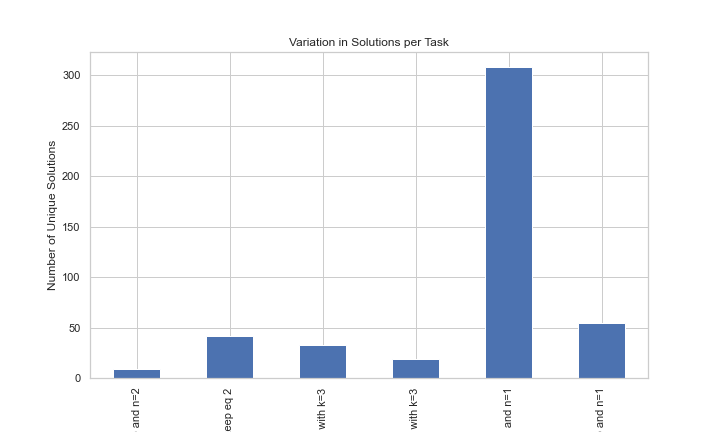
\includegraphics[width=\textwidth]{../img/plot_solution_variations.png}
    \caption{}
    \label{fig:solution_variations}
\end{figure}
Figure \ref{fig:solution_variations} showcases a bar chart detailing the diversity of solutions per task. Each bar corresponds to a specific task, with the height representing the number of unique solutions that successfully solved the task. This chart effectively conveys the variability and complexity of solutions across different tasks, illustrating tasks that exhibit a higher degree of solution diversity.

\begin{figure}
    \centering
    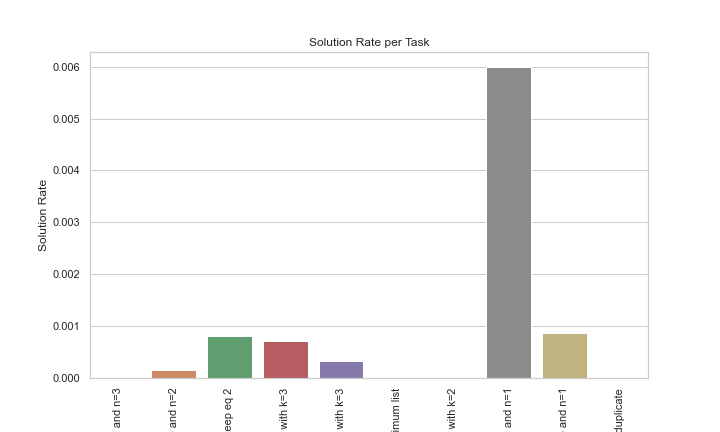
\includegraphics[width=\textwidth]{../img/plot_solution_rate_per_task.png}
    \caption{}
    \label{fig:solution_rate_per_task}
\end{figure}
In Figure \ref{fig:solution_rate_per_task}, a bar chart is used to depict the solution rate for each task. The tasks are displayed along the x-axis, and the corresponding solution rates are plotted on the y-axis. This chart provides a clear comparison of the relative difficulty or tractability of each task within the dataset, as indicated by the proportion of successful solutions.


\begin{figure}
    \centering
    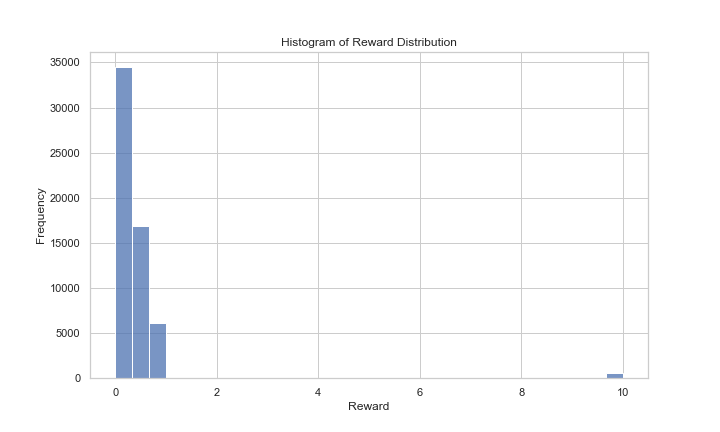
\includegraphics[width=\textwidth]{../img/plot_reward_distribution.png}
    \caption{}
    \label{fig:reward_distribution}
\end{figure}
Figure \ref{fig:reward_distribution} displays a histogram of the reward distribution across all attempts. This graph offers insights into the typical reward outcomes, including the most common reward values and the spread of rewards. The x-axis indicates the reward magnitude, while the y-axis shows the frequency of each reward range, highlighting the central tendency and variability of the reward structure.

\begin{figure}
    \centering
    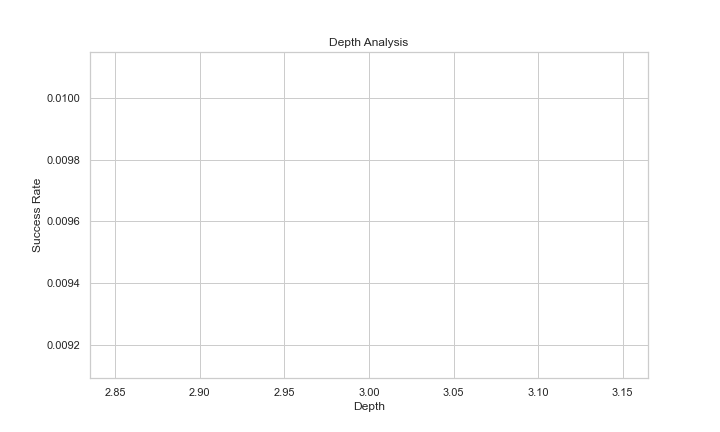
\includegraphics[width=\textwidth]{../img/plot_depth_analysis.png}
    \caption{}
    \label{fig:depth_analysis}
\end{figure}
Figure \ref{fig:depth_analysis} is a line chart that explores the relationship between the depth of the programs and their success rates. The depth of a program is plotted on the x-axis, and the corresponding success rate is indicated on the y-axis. This analysis is crucial for understanding how the complexity of a program, as measured by its depth, affects its likelihood of successfully solving a task.

\begin{figure}
    \centering
    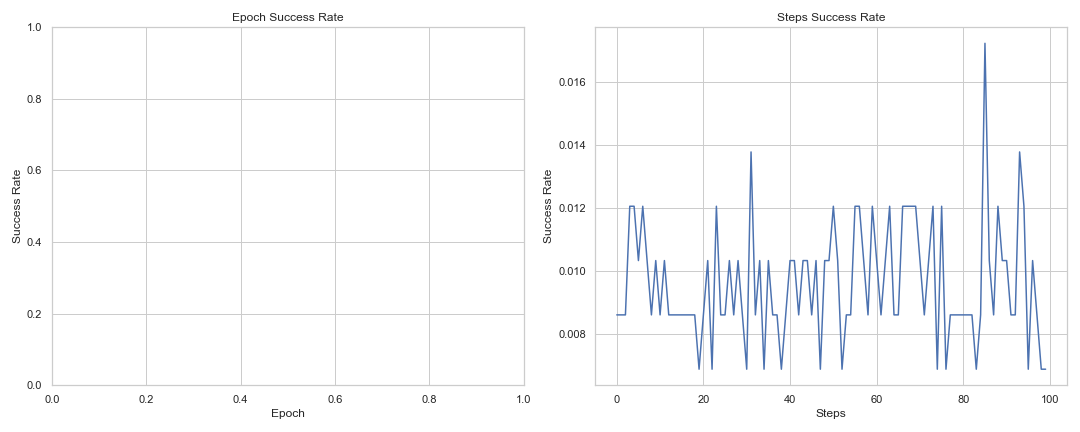
\includegraphics[width=\textwidth]{../img/plot_epoch_steps_analysis.png}
    \caption{}
    \label{fig:epoch_steps_analysis}
\end{figure}

In Figure \ref{fig:epoch_steps_analysis}, two line charts are presented, one for the success rate over different epochs and the other for the success rate over a number of steps. These charts elucidate the progression of success rates over time (epochs) and the iterative solving process (steps), providing a dynamic view of the learning or problem-solving efficiency.

\begin{figure}
    \centering
    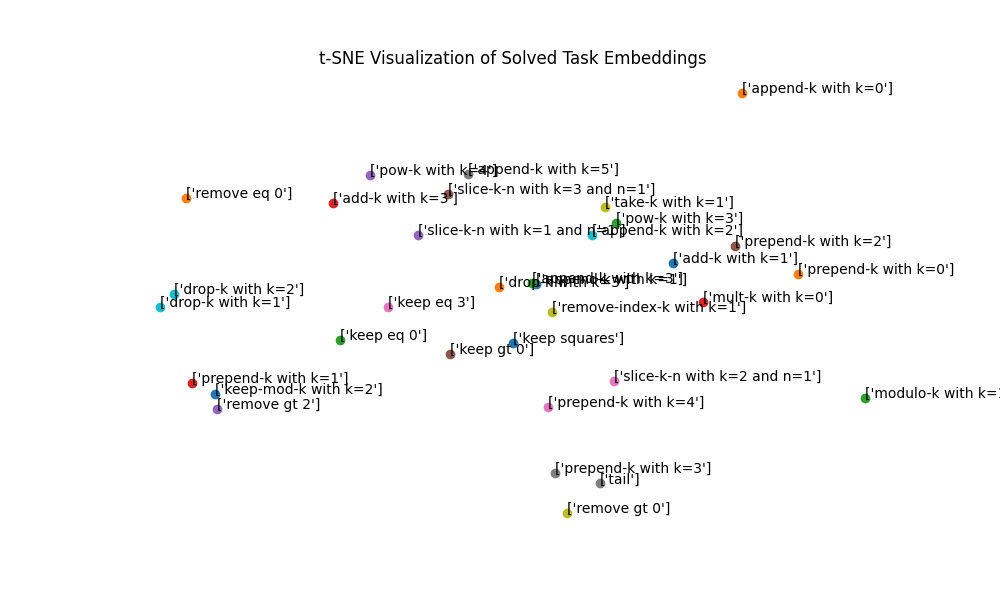
\includegraphics[width=\textwidth]{../img/task_embeddings.png}
    \caption{}
    \label{}
\end{figure}




    







\subsection{Discussion}

Time comparison
It is somewhat difficult to compare my method with other approaches.
other approaches parallelize processes on multiple CPUs (20-100 CPUs in DC). It takes DC 10 wake-sleep cycles to converge in the list domain
- I instead am working on one GPU (with possible interruptions from other users on the cluster)
- they show that the refactoring algorithm (which i havent used) helps a lot in list processing tasks.
- In DeepSynth, they only count the time of search, not of querying the model. 
- In Gflownet-EM (and other GFN papers) they train on over 50.000 epochs for simple problems. So this approach takes long to converge, but we reap the benefits at inference time. 


\begin{itemize}
    \item discuss the variable/ non variable batching. (credit assignment.)
    \item mode seeking. difficulty of broad and focussed modes. 
    \item MAP want to find the best (and shortest, given the right inductive bias) solution to the program. MLE tries to find a posterior distribution, i.e. all solutions of the task. (syntactically different but semantically equivalent solutions. Why do you think this would be necessary in real life. Argue.) 
    \item Perhaps in this toy scenario we don't necessarily need many solutions, but in general we do. 
    \item Make the network choose where to expand (not DFS). Note that we are not going through the CFG DFS, but creating the AST with DFS
    \item Temporal dimension? (GLOM includes time)
    \item in DeepSynth and DreamCoder, because of outsourcing the weights to the PCFG, they can parallelise it to CPUs rather than using more expensive GPU time. 
    \item Talk about batches and how it might speed up the process but perhaps make it more difficult to learn?
    \item What should be the best order of solving tasks? should we try to solve a certain task for x amount of time and then move on to the next? curriculum learning? 
    \item infer the cfg rather than have it as given. in DC they use variable scoping rules to determine which primitives are allowed, in deepsynth they just create a cfg because its faster. 
    \item Reward should be learnt (Energy based model). Where does the brain get it from?
    \item Is Levenshtein a reasonable reward? think about computational complexity (Kologorov complexity) 
\end{itemize}


\subsubsection{Complexity Analysis}

The time complexity for encoding an IO pair is \(\mathcal{O}(n)\), where \(n\) is the length of the IO pair. 

Similarly, the RuleEncoder's time complexity is \(\mathcal{O}(n)\) where \(n\) is the number of rules.

In each step of the trajectory, I embed the task and the current state, and use the transformer to construct the trajectory until completion. 

The transformer's complexity is \(O(num\_layers \times (d_{model}^2 \times n_{seq} + n_{seq}^2 \times d_{model}))\), where \(num\_layers\) is the number of layers, \(d_{model}\) is the model dimension, and \(n_{seq}\) is the sequence length.

The linear layers within the forward policy $\pi_\theta$ and partition function $Z_\theta$ have a complexity of \(O(d_{model}^2)\) due to the matrix multiplication involved.

The overall time complexity of a forward pass through the 'GFlowNet' model is dominated by the transformer's complexity, which is \(O(num\_layers \times (d_{model}^2 \times n_{seq} + n_{seq}^2 \times d_{model}))\).


Since I have linearized the construction procedure, I reconstruct the list back to AST format and then evaluate the tree to get the program output.

The reconstruction and evaluation are both recursive processes that depend on the depth of the tree and number of arguments in each partial program. 
The worst-case complexity of program reconstruction, as well as the evaluation can be approximated as \(O(k^d)\), where \(d\) is the depth of the recursion, which corresponds to the length of the program list, and \(k\) is the average number of arguments for each function in the program. However, this worst-case scenario is likely to be rare in practical applications, where both \(d\) and \(k\) are bounded and relatively small. In these experiments only one argument per function is allowed.

Subsequently, I compute the reward.

The Levenshtein edit distance algorithm, when implemented using dynamic programming, has a time complexity of 
$\mathcal{O}(m \times n)$, where $m$ and  $n$ are the lengths of the two input strings.



\subsubsection{Limitations}

\subsubsection{Future Work}
\begin{itemize}
    \item Sub-trajectory balance
    \item Learning from dataset of good programs (akin to someone telling you a solution)
    \item Train from middle of states
    \item Train backward policy, then we can also see finished states and predict trajectories that led to them
    \item caching evaluations, bottom-up
    \item we could let automate how long to train. if it is solving the task in 100 consecutive e steps and also in m stepts, it could also just move on. 

\end{itemize}












\subsection{Conclusion}
\begin{itemize}
    \item The conclusion here is that GFN is a viable method for program synthesis which could replace models such as DC. 
    \item 
\end{itemize}

\subsection{Discussion}
\begin{itemize}
    \item Scaling the model (How does the model scale with larger CFGs?)
    \item We need to show that with abstraction, we could theoretically scale
    \item Scaling neural search paper
    \item how would it work using GFNs
    \item how would it work if we use abstraction like in DC? 
    \item What have we learnt from autopoeisis, FEP, self-organisation, etc. Is my general approach a viable explanans to the eplanadum in question: is the conceptual world constructed by the same process we see in nature etc.
    \item If so, are programs a good representation?
    \item What are the general pitfalls of symbols?  (maybe this should go in general discussion)
    \item other models like GNN, other AST representations, other spaces, hyperbolic, etc. 
\end{itemize}



\subsubsection{Comparison to other approaches}

Previously, techniques in approximate Bayesian inference, have been applied to deal with the difficult marginalization term.

Variational Inference (VI) is a strategy that leverages a simpler distribution \( q(z | x) \)  to approximate a more complex target distribution. This is achieved by minimizing the Kullback-Leibler (KL) divergence [definition?] between the true distribution and its approximation.

\[
    D_{KL}[q_(z|x) || p_(z|x)]
\]

The approximation can be optimized by increasing the Evidence Lower Bound (ELBO) by:

\begin{equation}
\text{ELBO} = E_{q(z|x)}[\log p(x|z)] - D_{KL}(q(z|x) || p(z|x))
\end{equation}
Where \( E_{q(z|x)} \) denotes the expectation under the recognition density \( q \).

In the context of \emph{amortized} VI, computation of the variational parameters \( \phi \) is shared across multiple data points. Traditional VI might determine a unique set of variational parameters \( \phi_i \) for each data point \( x_i \), which is computationally intensive. Amortized VI, however, leverages a function (commonly a neural network) to compute the variational parameters \( \phi \) for any data point \( x \) in a single pass, enhancing efficiency. In other words, we parameterize the recognition density. 

this aligns with the free energy principle formulation [show that.]
maximizing the evidence lower bound (ELBO), is equivalent to the negative free energy. 


Amortized variational inference refers to the use of a parameterized function (e.g., a neural network) to approximate the posterior distribution in a variational Bayesian setting, where the parameters are learned once and can be used to infer the posterior for any given data point without retraining. It is "amortized" because the cost of learning the inference model is spread over all the data points it is used on.

GFlowNets relate to amortized variational inference in the sense that they learn a policy network that can generate samples for any given reward function without having to solve a new optimization problem for each sample. This is similar to how an amortized inference model can be applied to new data without additional optimization.

In both cases, the "amortization" allows for efficient inference or generation after the initial cost of learning the model. However, GFlowNets focus on learning to sample in proportion to a reward function, whereas amortized variational inference is concerned with approximating the posterior distribution of latent variables given observed data.





\begin{itemize}
    \item Relation to MDPs, POMDPs
    \item Relation to Reinforcement learning
    \item Relation to MCMC sampling
    \item Relation to Variational inference. 
\end{itemize}


variational approximation we need an ELBO but with GFNs we don't 









- **Hierarchical Models**: Both probabilistic programming and human cognition exploit hierarchical structures, where higher levels capture more abstract representations and lower levels deal with details. This facilitates learning and transfer of knowledge across different tasks and contexts. [introduce Compositional LVMs]

- **Active Inference**: Probabilistic programming in cognition implies that the brain is engaged in active inference, selecting actions based on their expected outcomes to minimize the divergence between predicted and actual states (akin to minimizing a cost function in a program). [we are learning an action policy]












A variety of techniques have emerged in the domain of program synthesis, [each with pros and cons].

Ullman et al. MCMC[source, definition] and Metropolis-Hastings[source, definition] \cite{ullman_theory_2012}. [include pros and cons]

% Example-based synthesis draws inspiration from how humans often learn—from examples. These methods generate programs by generalizing from provided instances, which mirrors pedagogical processes and experiential learning [source].

% Stochastic Search: By randomly exploring the space of possible programs, these methods mirror heuristic-based cognitive processes. Genetic algorithms, for instance, mimic evolutionary processes to evolve optimal or near-optimal solutions.

% Neural Program Synthesis: Neural networks, especially recurrent ones, have shown promise in generating programmatic structures. The parallels between neural networks and neural structures in the brain offer tantalizing possibilities for cognitive science.

% Program synthesis in its most general formulation is undecidable, which necessitates some form of search over the (possibly expanding) program space \cite{gulwani_program_2017} [reference to undecidability, size of program space etc.]. 

% A variety of statistical techniques have been proposed, ranging from evolutionary algorithms, 
% machine learning and genetic programming to MCMC sampling and probabilistic inference [source].  

% Machine learning techniques can be used to augment other search methodologies based on enumerative search or deduction by providing likelihood of various choices at any choice point. One such choice point is selection of a production for a non-terminal in a grammar that specifies the underlying program space. The likelihood probabilities can be function of certain cues found in the input-ouput examples provided by the user or the additionally available inputs [89]. These functions are learned in an offline phase from training data. 

% Genetic programming is a program synthesis method inspired by biological evolution [72]. It involves maintaining a population of individual programs, and using that to produce program variants by leveraging computational analogs of biological mutation and crossover. Mutation introduces random changes, while crossover facilitates sharing of useful pieces of code between programs being evolved. Each variant's suitability is evaluated using a user-defined fitness function, and successful variants are selected for continued evolution. The success of a genetic programming based system crucially depends on the fitness function. Genetic programming has been used to discover mutual exclusion algorithms [68] and to fix bugs in imperative programs [146] 

% MCMC sampling has been used to search for a desired program starting from a given candidate. The success crucially depends on defining a smooth cost metric for Boolean constraints. STOKE [124], a superoptimization tool, uses Hamming distance to measure closeness of generated bit-values to the target on a representative test input set, and rewards generation of (almost) correct values in incorrect locations. 

% Probabilistic inference has been used to evolve a given program by making local changes, one at a time. This relies on modeling a program as a graph of instructions and states, connected by constraint nodes. Each constraint node establishes the semantics of some instruction by relating the instruction with the state immediately before the instruction and the state immediately after the instruction [45]. 

% Belief propagation has been used to synthesize imperative program fragments that execute polynomial computations and list manipulations [62].

\cite{gulwani_program_2017}

ASTs
\cite{oliveira_abstract_2013}
\cite{zhang_novel_2019}












\subsubsection{Biological Plausibility}
\begin{itemize}
    \item Why are/ aren't types plausible? Related to categories?
    \item CFG? where does it come from?
    \item primitives?
\end{itemize}



\begin{itemize}
    \item How are programs represented (ASTs, GNNs, other ideas from different papers)
    \item Tree-Transformers
\end{itemize}











\begin{itemize}
    \item Loss optimality
    \item There is a trade-off between finding many programs rapidly, or fewer programs that are more likely to solve the problem.
    \item enumeration vs sampling
    \item They show that all sampling algorithms are either loss optimal or have infinite loss?
\end{itemize}











% \subsubsection{CFG} \label{subsubsec:cfg}

% \improvement[inline]{here we talk about the idea that our thoughts are constructed as a type of formal language. a LOT. not specifically programs yet.}


% \Gls{Context-Free Grammars} (CFGs) are essential in defining the syntactical structures of many formal languages [i dont like this sentence yet, general definition first?]. However, given the generative nature of CFGs, the space defined by even a modestly complex grammar can be immensely vast. Searching for a specific sentence within this space, or ensuring that a particular space is sufficiently explored, poses significant computational challenges. [reference to computational irreducibility, undecidability]

% We can formalize the notion of CFGs as follows:

% Let \( G = (N, \Sigma, P, S) \) be a Context-Free Grammar, where:


% % \begin{conditions*}
% %     N & \text{A finite set of non-terminal symbols}
% %     \Sigma & \text{A a finite set of terminal symbols with} N \cap \Sigma = \emptyset
% %     P & \text{A finite set of production rules, where each rule is of the form} N \rightarrow (N \cup \Sigma)^*
% %     S & \text{The start symbol, with} S \in N
% % \end{conditions*}

% \begin{itemize}
%     \item \( N \) is a finite set of non-terminal symbols.
%     \item \( \Sigma \) is a finite set of terminal symbols with \newline \( N \cap \Sigma = \emptyset \)
%     \item \( P \) is a finite set of production rules, where each rule is of the form \( N \rightarrow (N \cup \Sigma)^* \)
%     \item \( S \) is the start symbol, with \( S \in N \)
% \end{itemize}

% Given such a CFG, the derived sentence space \( \Pi(G) \) is the set of all possible strings (or sequences of symbols) derivable from \( S \).

% Given a Context-Free Grammar \( G \) and a defined objective function \( f \) that maps any program \( p \in \Pi(G) \) to a real value representing its desirability or fitness:

% Find \( p^* \) such that:
% \[ p^* = \arg\max_{p \in \Pi(G)} f(p) \]

% In other words, the problem is to locate a program \( p^* \) within the vast program space \( \Pi(G) \) defined by \( G \) that maximizes (or, alternatively, minimizes) the objective function \( f \).

% [meeting a specification]


% % 3.2 Non-Linearity and Discontinuities

% The mapping between programs and their fitness as defined by \( f \) might be non-linear with multiple local maxima, making search strategies based on gradient ascent or other linear heuristics suboptimal.

% % 3.3 Generalization vs Specification

% While CFGs provide a generalized representation of possible programs, the objective function might lead to highly specialized solutions. Balancing between the two is non-trivial.

% 3.4 Syntactic vs Semantic Validity

% A CFG ensures syntactic validity but does not guarantee semantic correctness. Ensuring that a program derived from a CFG is semantically meaningful or error-free in a given context is an additional layer of complexity.
























% \section{What's missing?}

% \begin{itemize}
%     \item nathaniel et al show quality vs quantity, sampling vs enumeration.
% \end{itemize}




% Although these models are great, their method reveals a foundational limitation: their heavy reliance on syntactical constraints. While these constraints are undoubtedly vital for ensuring the correctness of generated programs, they do not necessarily guarantee a deep understanding or utilization of semantic relationships within the code. 
% A lot of information may be lost, by disregarding the semantic relationships. As we have seen in [reference LLMs], there seems to be a semantic grammar on top of the syntactical structure of the language which we may be able to leverage.
% This has been criticized in [cite all the relevant papers (using GNNs, etc. ) also Kim's neural PCFG].
% Perhaps we can utilise transformers to learn a "program space", a kind of neural probabiilistic context-free grammar

% - we could imagine a program space in which symmetries [reference] and so on could be leveraged. For example, one could argue that "\(+\)" is to "\(-\)" as "\(\div\)" is to "\(\times\)", and anyways once we create programs which really represent actual concepts, the same regularities should be systematically compressed.

% Perhaps the attention mechanism, as seen in transformers, provides a potential solution to this limitation. 
% I.e. if we can amortize the cost of learning, we can get a good inference machine, which samples according to the posterior.


% % The overall objective is to learn the \gls{domain specific language}, and also to learn how to navigate through it, in order to construct programs that match a certain specification.
% - taking the approach of world model and inference model.
% - at the moment i am only focussing on generating programs, not improving the DSL, using abstractions.







% GFlowNets can be seen as extending the already rich family of **amortized variational inference** methods, more specifically amortized hierarchical variational inference, where there are several latent variables $s_1, s_2, \ldots$ and they are hierarchically organized so that when we generate an object $x$ we start by sampling $s_1$, then $s_2|s_1$, then $s_3|s_2$, etc and then convert the last $s_{n-1}$ into $x=s_n$ with a model $P(s_1,s_2,\ldots,s_{n-1},x)=P(x|s_{n-1})P(s_{n-1}|s_{n-2})\ldots P(s_2|s_1)$. As discussed in [[7]](https://www.notion.so/The-GFlowNet-Tutorial-95434ef0e2d94c24aab90e69b30be9b3?pvs=21) and [[9]](https://www.notion.so/The-GFlowNet-Tutorial-95434ef0e2d94c24aab90e69b30be9b3?pvs=21), the sequence $\tau=s_1,\ldots,s_{n-1},x$ corresponds to the GFlowNet trajectory $\tau$, with $P_F(\tau)=P(x|s_{n-1})\ldots P(s_2|s_1)$. As with other variational inference approaches one also learns an inference machine $Q(\tau|x)$ which corresponds to $P_B(\tau|x)$ in GFlowNets. With variational method we also have a marginal data distribution (which we could denote $Q(x)$) that with GFlowNets corresponds to the normalized reward function $R(x)/Z$ that can be queried as needed by the training procedure (unlike a fixed dataset). Another difference is that variational methods are trying minimize the reverse KL divergence between $Q$ and $P$ (or using importance sampling, the forward KL) whereas GFlowNets are trained with a diversity of losses, e.g. corresponding to something like $(\log Q(\tau) - \log P(\tau))^2$ with Trajectory Balance, that open the possibility of offline training (with trajectories $\tau$ sampled from a distribution different from the online samples from $Q$). In [[9]](https://www.notion.so/The-GFlowNet-Tutorial-95434ef0e2d94c24aab90e69b30be9b3?pvs=21), we show that when a GFlowNet is trained with trajectory balance on-policy, the expected gradient is the same as with variational inference and the reverse KL, but the variance is different (and the trajectory balance gradient is equivalent to using a variance reduction trick, compared with regular variational inference). The typical variational inference objective (the ELBO or reverse-KL) leads to mode-following (focussing on one mode) and the forward KL leads to mean-following (overly conservative, sampling too broadly) and annoying variance when implemented with importance sampling. Instead the off-policy GFlowNet objectives (e.g., with a tempered version of $P_F$ as training policy) seem to strike a different balance and tend to recover more of the modes without the down-side of the forward-KL variational inference variants (mean-following and high variance gradients). Another difference is that GFlowNets can learn flows and conditional flows, which correspond to marginalized quantities, as discussed [above](https://www.notion.so/The-GFlowNet-Tutorial-95434ef0e2d94c24aab90e69b30be9b3?pvs=21).




\begin{itemize}
    \item Robustfill
    \item DeepCoder
    \item Etc.
    \item Paved the way in a coubple of different ways, etc.
\end{itemize}















% \begin{figure}
%     \centering
%     \begin{tikzpicture}[
%       node distance = 2cm,
%       auto,
%       block/.style = {circle, draw, font=\sffamily\Large\bfseries},
%       line/.style = {draw, -latex}
%     ]
    
%     % Nodes
%     \node [block] (S) {S};
%     \node [block, below left of=S] (R1) {R};
%     \node [block, below right of=S] (T1) {T};
%     \node [block, below left of=R1] (R2) {R};
%     \node [block, below right of=R1] (T2) {T};
%     \node [block, below right of=R2] (a) {a};
%     \node [block, right of=a] (b) {b};
    
%     % Paths
%     \path [line] (S) -- node {f(R,T)} (R1);
%     \path [line] (S) -- node {g(T)} (T1);
%     \path [line] (R1) -- node {f(R,T)} (R2);
%     \path [line] (R1) -- node {g(T)} (T2);
%     \path [line] (T2) -- node {a} (a);
%     \path [line] (T2) -- node {b} (b);
    
%     % DFS, BFS, A* paths (without specific details)
%     \draw [red, thick, dashed] (S) to [bend left] (R2);
%     \draw [blue, thick, dashed] (S) to [bend right] (b);
%     \draw [green, thick, dashed] (S) to [bend right] (T2);
    
%     \end{tikzpicture}
%     \caption{Illustration of the tree of leftmost derivations.}
%     \end{figure}


    % \begin{figure}
    %     \centering
    %     \begin{tikzpicture}[
    %       node distance = 1.5cm,
    %       auto,
    %       block/.style = {circle, draw, fill=orange, font=\sffamily\Large},
    %       line/.style = {draw, -latex},
    %       dashedline/.style = {dashed, -latex}
    %     ]
        
    %     % Legend
    %     \node [draw, rectangle, minimum width=3cm, minimum height=2cm, font=\small] at (0,5) {legend};
    %     \node [font=\small] at (0,4.5) {--- semantic equivalence};
    %     \node [font=\small] at (0,4) {⊔ nondeterministic choice};
        
    %     % Nodes for (A)
    %     \node [block] at (0,2) (A1) {+};
    %     \node [block, below left of=A1] (A1L) {5};
    %     \node [block, below right of=A1] (A1R) {x};
        
    %     % Nodes for (B)
    %     \node [block] at (4,2) (B1) {+};
    %     \node [block, below left of=B1] (B1L) {5};
    %     \node [block, below right of=B1] (B1R) {x};
        
    %     % Paths for (A)
    %     \draw [line] (A1) -- (A1L);
    %     \draw [line] (A1) -- (A1R);
        
    %     % Paths for (B)
    %     \draw [dashedline] (B1) -- (B1L);
    %     \draw [dashedline] (B1) -- (B1R);
        
    %     % ... continue for other nodes and paths ...
        
    %     \end{tikzpicture}
    %     \caption{Refactorings and data structure.}
    %     \end{figure}



    \begin{figure*}[htbp]
        \centering
        \begin{adjustbox}{width=\textwidth}
            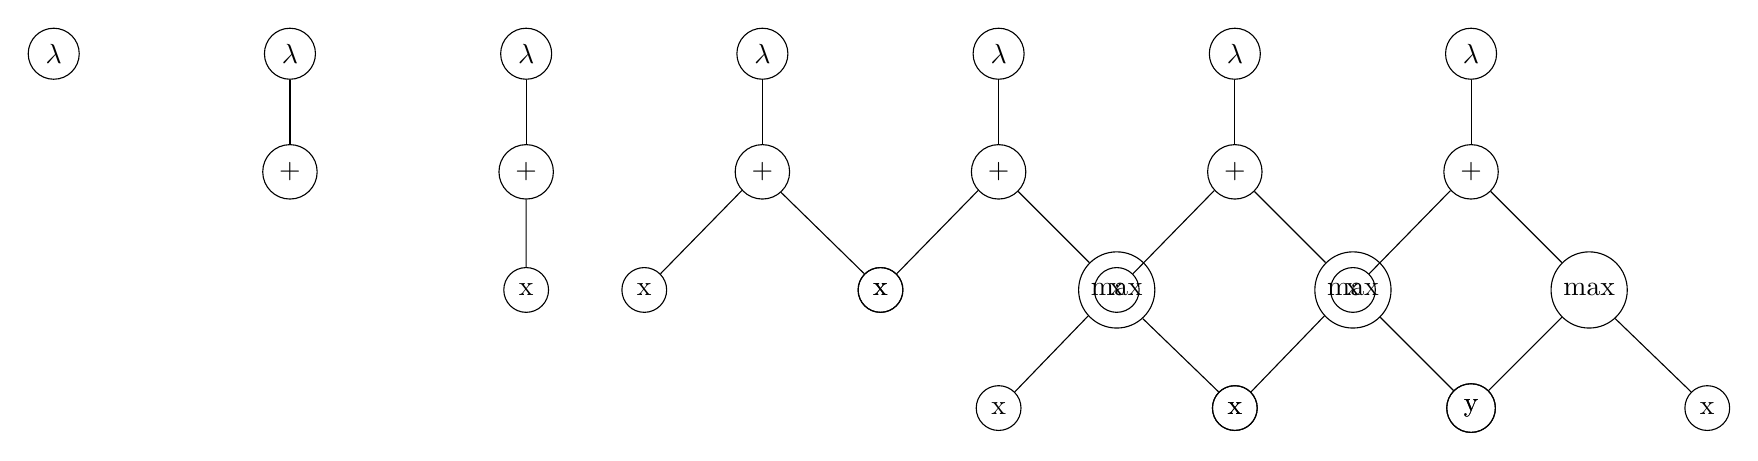
\begin{tikzpicture}[level distance=1.5cm,
                level 1/.style={sibling distance=6cm},
                level 2/.style={sibling distance=3cm},
                every node/.style={circle, draw}]
            
            \node at (-9,0) {$\lambda$};
            \node at (-6,0) {$\lambda$}
                child {node {+}};
            \node at (-3,0) {$\lambda$}
                child {node {+}
                    child {node {x}}
                };
            \node at (0,0) {$\lambda$}
                child {node {+}
                    child {node {x}}
                    child {node {x}}
                };
            \node at (3,0) {$\lambda$}
                child {node {+}
                    child {node {x}}
                    child {node {max}
                        child {node {x}}
                        child {node {x}}
                    }
                };
            \node at (6,0) {$\lambda$}
                child {node {+}
                    child {node {x}}
                    child {node {max}
                        child {node {x}}
                        child {node {y}}
                    }
                };
            \node at (9,0) {$\lambda$}
                child {node {+}
                    child {node {x}}
                    child {node {max}
                        child {node {y}}
                        child {node {x}}
                    }
                };
            
            % % Second tree sequence (Figure 6)
            % \node at (-3,-5) {+};
            % \node at (0,-5) {+}
            %     child {node {pow}};
            % \node at (3,-5) {+}
            %     child {node {pow}
            %         child {node {y}}
            %     };
            % \node at (6,-5) {+}
            %     child {node {pow}
            %         child {node {y}}
            %         child {node {x}}
            %     };
            % \node at (9,-5) {+}
            %     child {node {pow}
            %         child {node {y}}
            %         child {node {x}}
            %     }
            %     child {node {3}};
            
            \end{tikzpicture}
        \end{adjustbox}
        \caption{Creation of trees showing the construction process.}
    \end{figure*}
    
    
    

    % todo: table of parameters and syntactic constraints (appendix)
















    \begin{figure*}[htbp]
        \centering
        \begin{adjustbox}{width=\textwidth}
            \begin{tikzpicture}[
                node distance=2cm, 
                auto, 
                thick,
                box/.style={
                    rectangle,
                    rounded corners,
                    draw=black, 
                    align=center,
                    drop shadow,
                    minimum height=1cm,
                    minimum width=2cm
                },
                arrow/.style={
                    ->,
                    -{Stealth[length=10pt]}
                }
            ]
            
                % Nodes
                \node[box, fill=yellow!50] (task) {Task};
                \node[box, fill=yellow!70, right=3cm of task] (ioencoder) {IOEncoder};
                \node[box, fill=blue!20, below=1cm of task] (state) {State};
                \node[box, fill=blue!50, right=3cm of state] (ruleencoder) {RuleEncoder};
                
                % Positioning the Transformer node in between IOEncoder and RuleEncoder
                \coordinate (middle) at ($(ioencoder.east)!0.5!(ruleencoder.east)$);
                \node[box, fill=green!20, right=3cm of middle] (transformer) {Transformer};
                
                % Nodes for FORWARD and Z at 45 degree angles
                \node[box, fill=purple!30, above right=0.5cm and 2cm of transformer] (forward) {FORWARD};
                \node[box, fill=purple!50, below right=0.5cm and 2cm of transformer] (z) {Z};
            
                % Edges
                \draw[arrow] (task) -- (ioencoder);
                \draw[arrow] (state) -- (ruleencoder);
                \draw[arrow] (ioencoder) -- (transformer);
                \draw[arrow] (ruleencoder) -- (transformer);
                \draw[arrow] (transformer) -- (forward);
                \draw[arrow] (transformer) -- (z);
            
            \end{tikzpicture}
        \end{adjustbox}
        \caption{Insert explanation + maybe change task to an actual task; same with state; maybe also show the forward and Z output better.}
        \label{ref:model_diagram}
    \end{figure*}
    
    
    
    